\documentclass[a4paper]{article}

\usepackage{xcolor}
\usepackage{fancyheadings}
\usepackage{listings}
\usepackage{graphicx}
\usepackage[section]{placeins}
\usepackage{hyperref}
\usepackage[utf8]{inputenc}

% colors
\definecolor{mygreen}{rgb}{0,0.6,0}
\definecolor{mygray}{rgb}{0.5,0.5,0.5}
\definecolor{myblue}{rgb}{0,0,0.5}
\definecolor{mymauve}{rgb}{0.58,0,0.82}

% hyperref configuration
\hypersetup{
    colorlinks,
    linkcolor={mymauve},
    citecolor={myblue},
    urlcolor={myblue}
}

% Code listing configuration
\lstset{
  basicstyle=\footnotesize,        % the size of the fonts that are used for the code
  commentstyle=\color{mygreen},    % comment style
  keepspaces=true,                 % keeps spaces in text, useful for keeping indentation of code (possibly needs columns=flexible)
  keywordstyle=\color{blue},       % keyword style
  language=Python,                 % the language of the code
  morekeywords={interface,abstract,static}, % if you want to add more keywords to the set
  %numbers=left,                    % where to put the line-numbers; possible values are (none, left, right)
  numbersep=5pt,                   % how far the line-numbers are from the code
  numberstyle=\tiny\color{mygray}, % the style that is used for the line-numbers
  stringstyle=\color{mymauve}      % string literal style
}

% TODO command
\newcommand{\todo}[1]{\textcolor{red}{[#1]}\\}

% New custom label command
\makeatletter
\newcommand{\customlabel}[2]{%
   \protected@write \@auxout {}{\string \newlabel {#1}{{#2}{\thepage}{#2}{#1}{}} }%
   \hypertarget{#1}{#2}
}
\makeatother

% requirements
\newcounter{reqcount}
\newcommand{\requirement}[2]{%
  \item \refstepcounter{reqcount}\customlabel{req:#1}{\textbf{Eis \thereqcount}}: #2
}

\newcommand{\reqref}[1]{\ref{req:#1}}

% questions
\newcommand{\question}[1]{
  \subsubsection*{#1}
  \pdfbookmark[2]{#1}{question:#1}
}

% code in text
\newcommand{\code}[1]{\lstinline[columns=fixed]{#1}}

% heading
\lhead{Open Universiteit}
\chead{IM0102, Design patterns}
\rhead{Eindopdracht}

\begin{document}
\pagestyle{fancy}

\section*{Studentgegevens}
    \begin{description}
        \item [Cursuscode] IM0102
        \item [Opdracht] Jabberpoint Inhoudsopgave
        \item [Naam] Daniel S. C. Schiavini
        \item [Studentnummer] 851102873
    \end{description}

\section*{Aanpak}
    De oorspronkelijke bedoeling was om deze opdracht uit te voeren in een team met een andere student.
    Echter, er was geen andere student beschikbaar met een vergelijkbare tempo.
    Daardoor heb ik deze opdracht alleen uitgevoerd.

    Voordat ik wist dat ik de opdracht alleen mag uitvoeren, had ik al een Git repository gemaakt.
    Ik heb de repository zo geconfigureerd dat dit document automatisch wordt gebouwd door het gebruik van TravisCI.
    Zodra een nieuwe versie van het rapport naar GitHub wordt gepushed, draait een script dat het PDF-bestand maakt.
    Het script bouwt ook Jabberpoint, draait unit tests, en als alles gelukt is wordt ook een JAR-bestand gemaakt.
    In de master branch hangt een deployment vast dat het PDF en JAR naar \href{https://github.com/DanielSchiavini/design-patterns-assignment/tree/gh-pages}{GitHub pages} publiceert.
    Deze automatisering is iets minder nodig zonder team, maar het is nog steeds wel nuttig.

    Jabberpoint had nog geen geautomatiseerde tests en omdat ik dat belangrijk vind, heb ik van tevoren JUnit tests geschreven.
    Echter niet alle klassen waren testbaar -- TravisCI draait in een Linux-container waarin de Graphic Java-klassen niet gecreëerd kunnen worden.
    Ik had niet genoeg tijd had om dit probleem op te lossen, daarom heb ik alleen tests geschreven voor de domein- en accessor-klassen.

    Het schrijven van de tests was een goede hulpmiddel om Jabberpoint te leren kennen en om het probleemanalyse van de volgende sectie uit te voeren.

\section{Probleemanalyse}
    \label{sec:probleemanalyse}
    Om het probleem te analyseren kunnen we het beste de opdracht in eisen omschrijven:

    \begin{itemize}
        \requirement{toevoegen}{De gebruiker moet één of meer slides met inhoudsopgaven kunnen toevoegen aan een presentatie.}
        \requirement{tonen}{Een inhoudsopgave-slide moet alle onderwerpen van de presentatie tonen.}
        \requirement{samenvoegen}{Het onderwerp moet slechts eenmaal worden getoond wanneer meerdere slides achter elkaar hetzelfde onderwerp hebben.}
        \requirement{updaten}{De inhoudsopgave moet automatisch worden geüpdatet wanneer slides worden toegevoegd of verwijderd.}
        \requirement{titel}{De titel moet als onderwerp worden gebruikt wanneer een slide geen onderwerp heeft (\textbf{aanname}).}
        \requirement{onderwerpen}{Het onderwerp mag op slides worden getoond, behalve in de inhoudsopgave (optioneel).}
        \requirement{volgnummers}{De onderwerpen in de inhoudsopgave mogen volgnummers krijgen (optioneel).}
        \requirement{aanduiding}{Het onderwerp van de slide die na een inhoudsopgave komt, mag een speciale aanduiding krijgen (i.e. een alternatieve letterstijl) (optioneel).}
        \requirement{stijl}{De stijl van de inhoudsopgave is vrij te bepalen.}
    \end{itemize}

    \todo{Create PR for \reqref{volgnummers} and \reqref{onderwerpen}.}

    De opdracht om een inhoudsopgave te implementeren in Jabberpoint is best interessant.
    Om een inhoudsopgave te tonen, is kennis nodig van de hele presentatie.
    Een verandering in elke slide kan invloed hebben op alle inhoudsopgaven.
    Deze circulaire afhankelijkheid maakt de opdracht uitdagend.

\section{Ontwerp}
    Het onderwerp zoals geïmplementeerd verandert weinig van het originele Jabberpoint-ontwerp.
    Er is een nieuwe klasse toegevoegd voor de inhoudsopgaven, namelijk \code{TableOfContentsSlide}.
    Deze nieuwe klasse is een sub-klasse van \code{Slide}.

    Het grootste verschil tussen de klassen is dat de inhoudsopgave kennis moet hebben van de hele presentatie.
    Daardoor krijgt een \code{TableOfContentsSlide} een referentie naar de presentatie in de constructor.

    Zodra de inhoudsopgave getekend gaat worden, worden de presentatie onderwerpen gelezen en wordt een nieuwe lijst van slide-items gemaakt.
    Daartoe kunnen wij de bestaande methoden van de \code{Slide} klasse gebruiken.
    Omdat er geen speciale stijl-eisen zijn voor de inhoudsopgave, kunnen wij eenvoudig de al ingebouwde levels gebruiken om de stijl te bepalen.

    De aangepaste klassendiagram wordt in figuur~\ref{fig:design} getoond.
    \begin{figure}[!htb]
     \caption{
        Klassendiagram voor de domein-objecten.\label{fig:design}
        Sterren geven de nieuwe klasse en methoden aan.
        \todo{Add presentation attribute to TableOfContents}
     }
     \centering 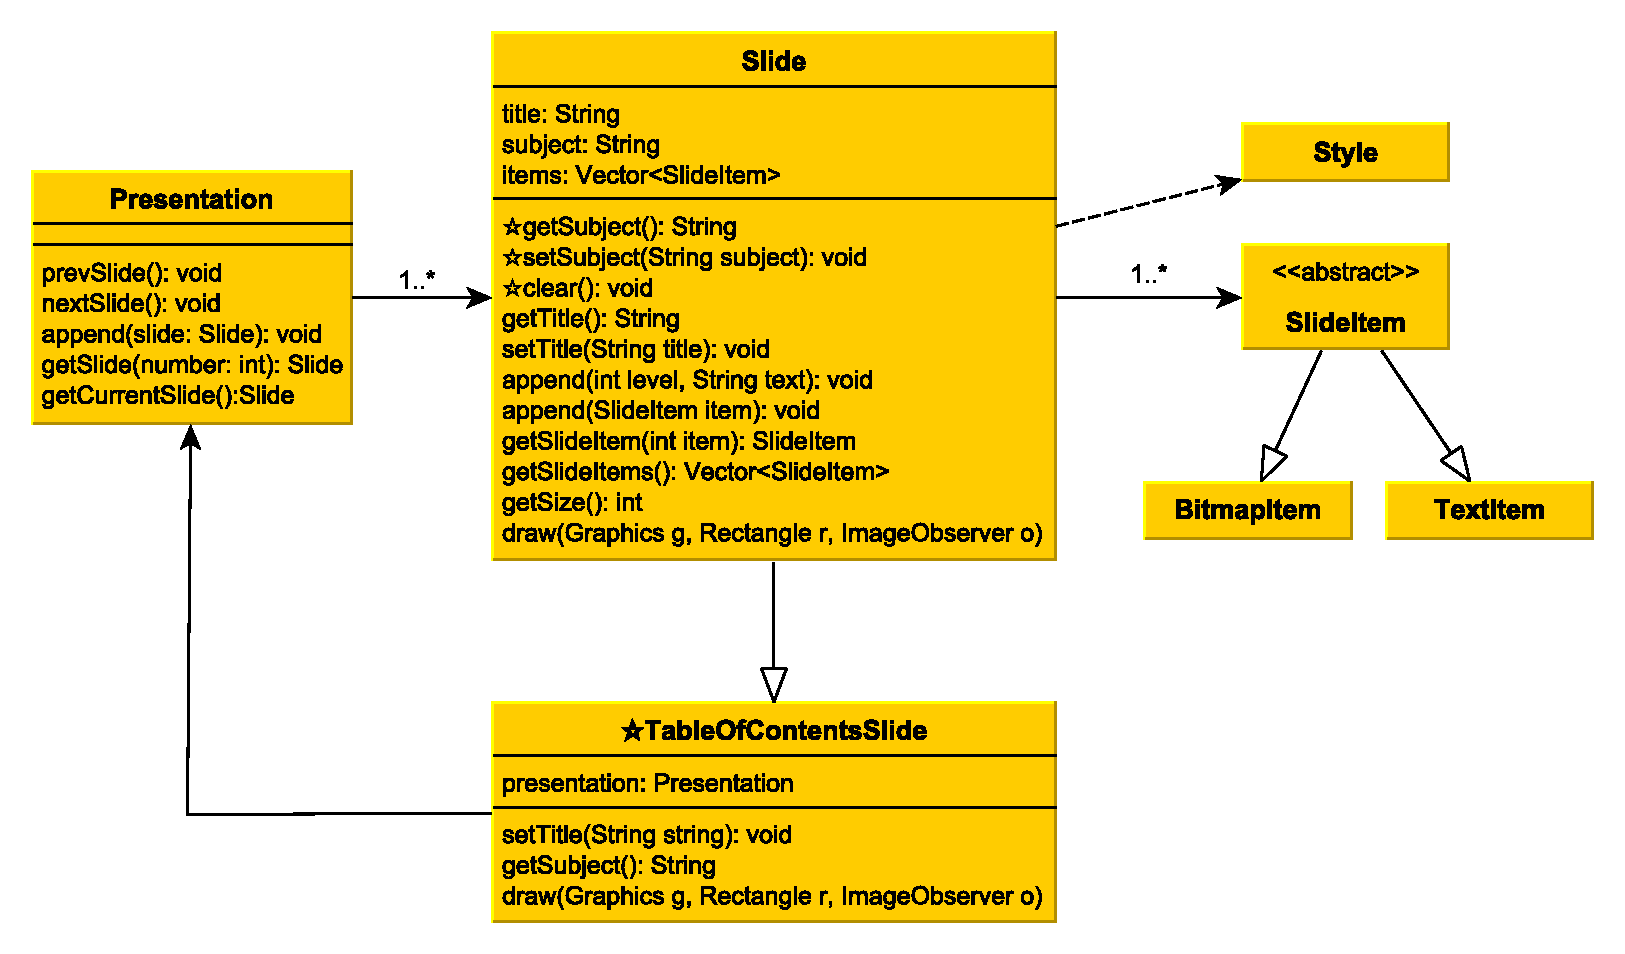
\includegraphics[width=\textwidth]{Diagrams/design.pdf}
    \end{figure}

    Het voordeel van dit onderwerp is dat er vrij weinig hoeft te veranderen.
    De Accessor-klassen krijgen de extra verantwoordelijkheid om de slide-objecten te maken en te schrijven.
    Voor de rest van de code is een inhoudsopgave een normale slide die zijn eigen content genereert.
    Accessor-klassen mogen zelf bepalen of er een referentie wordt opslagen naar een inhoudsopgave, of een lijst van de inhoud van de slides.

    Voor de implementatie van de \code{draw} methode was een manier nodig om alle eerdere slide-items te verwijderen.
    Het is natuurlijk ook mogelijk om de \code{items} attribuut rechtstreeks te veranderen (zelfs een super-klasse);
    maar het is in Java nooit verstandig om attributen van andere klassen te veranderen.
    Daarvoor komt een nieuwe \textbf{protected} methode \code{clear} in de slide.
    De attributen van \code{Slide} zijn \textbf{private} geworden.

    Het is verstandig om software te implementeren in de meest simpele manier, en dan itereren om deze te verbeteren.
    Daarom vind ik dat het bij de opdracht past om een aantal verbeteringen ook door te voeren.
    Dit wordt verder uitgelegd in sectie~\ref{sec:keuzen}.

    \subsection{Traceerbaarheid van eisen}
        In deze sectie geef ik onderdelen van het ontwerp aan die verantwoordelijk zijn om de eisen (zie sectie~\ref{sec:probleemanalyse}) te realiseren.
        Dit geeft dus de relatie tussen probleemanalyse en ontwerp.

        \begin{itemize}
            \item De \code{Accessor}-klassen zijn verantwoordelijk voor \reqref{toevoegen}.
            \item De \code{TableOfContentsSlide} klasse is verantwoordelijk voor: \reqref{tonen}, \reqref{samenvoegen},
                \reqref{updaten}, \reqref{titel}, \reqref{volgnummers}, \reqref{aanduiding} en \reqref{stijl}.
            \item De \code{Slide} klasse is verantwoordelijk voor: \reqref{onderwerpen}.
        \end{itemize}


\section{Keuzen}\label{sec:keuzen}
    Klasse \code{TableOfContentsSlide} is uiteraard verantwoordelijk voor het genereren van de inhoudsopgave.
    Daarbij hebben we de optie om de slide-items die al geïmplementeerd zijn te hergebruiken.
    Het is dus logisch om de software zo optimaal mogelijk te hergebruiken, en niet alleen de slide-items maar ook het tekenen van deze items.
    De inhoudsopgave is in feite een slide die zijn eigen content genereert.
    
    In de rest van deze sectie gaan we een aantal vragen door die zijn opgeroepen tijdens het analyseproces.
    
    \question{Hoe moet de Slide klasse-structuur eruit zien?}
    Het is vanzelfsprekend dat \code{TableOfContentsSlide} een groot deel van de \code{Slide} code nodig heeft.
    Bij het analyseren van Jabberpoint heb ik gemerkt dat de nieuwe klasse eigenlijk \textit{alle} code moet gebruiken.
    Het enige onderdeel dat niet nodig is voor de inhoudsopgave is het nieuwe onderwerp-veld.
    
    Meestal als een variatie komt voor een bestaand concept, moet er een interface (of abstracte klasse) komen die het oude en het nieuwe concept implementeren.
    De rest van het systeem werkt dan met de interface en hoeft niets te weten van de exacte implementatie.
    Dit is hier ook het geval, de presentatie-klassen hoeven immers niet te weten of een slide een inhoudsopgave is of niet.
    
    We zouden dus \code{Slide} abstract kunnen maken en een nieuwe klasse maken die naast de bestaande methoden een onderwerp heeft.
    Als we echter denken aan wat voor andere soorten \code{Slide} er in de toekomst nog komen, is het aannemelijk dat deze ook in de inhoudsopgave moeten worden getoond.
    
    Een alternatief ontwerp is geïmplementeerd in \hyperlink{https://github.com/DanielSchiavini/design-patterns-assignment/pull/17}{PR \#17}.
    In deze PR heeft \code{Slide} geen items meer, maar alleen een titel en \code{draw}.
    Een extra klasse \code{ContentSlide} gemaakt die slide-items heeft.
    Hierin maakt de \code{TableOfContentsSlide} elke keer een nieuwe \code{ContentSlide}.
    Dit ontwerp is een geldig alternatief maar er staan niet veel voordelen tegenover de toegenomen complexiteit.
    De software wordt immers ingewikkelder en er moeten extra \textit{casts} worden uitgevoerd (\textit{code smells}).

    \todo{Add diagram}

    \question{Wanneer items genereren}
    De table of contents is in feite een slide met een inhoud die gegenereerd wordt.
    De vraag is wanneer deze generatie moet gebeuren.
    In het gepresenteerde ontwerp wordt de slide opnieuw gegenereerd in elke \code{draw}.
    
    Een alternatief zou zijn om een manier te implementeren om de \code{TableOfContentsSlide} te laten weten als iets verandert.
    Bijvoorbeeld de observable pattern zou hier gebruikt kunnen worden.
    
    Dat is echter niet nodig, de generatie is redelijk efficiënt, immers \code{draw} wordt alleen aangeroepen als de slide zichtbaar komt.
    \code{SlideViewerComponent} roept namelijk \code{repaint} aan wanneer de slide op het scherm komt.
    
    \question{Welke klasse is verantwoordelijk voor de onderwerpen?}
    De inhoudsopgave moet toegang krijgen tot een lijst van onderwerpen in de presentatie.
    In het ontwerp krijgt \code{TableOfContentsSlide} een referentie naar de presentatie, en is zelf verantwoordelijk om deze te lezen.
    En alternatief hierop is om de presentatie verantwoordelijk te houden voor de onderwerpen in de slides.
    \code{TableOfContentsSlide} zou dan een ontvangt dan een onderwerpen-lijst.

    De voordelen zijn:
    \begin{itemize}
        \item De inhoudsopgave hoeft niets te weten van de presentaties.
        \item De presentatie is verantwoordelijk om slides te lezen.
        \item De circulaire referentie wordt opgeheven.
        \item De lijst van onderwerpen kan tussen de verschillende inhoudsopgaven worden gedeeld.
    \end{itemize}

    De nadelen zijn:
    \begin{itemize}
        \item Er komt meer logica in de presentatie die alleen nodig is voor de inhoudsopgave.
        \item De inhoudsopgaven moeten nog steeds alle items doorlopen om te bepalen welk onderwerp het volgende is.
        \item De methoden die nodig zijn om het ontwerp te presenteren bestaan al in de presentatie.
        \item Het is conceptueel correct om een circulaire referentie te hebben, immers een inhoudsopgave moet de presentatie lezen.
        \item De presentatie klasse wordt nog complexer.
    \end{itemize}
    
    De keuze om de onderwerpenlijst in de inhoudsopgave te implementeren geeft dus een betere inkapseling.

    \question{UI-domein vermengeling}
    Het feite dat slides en slide-items verantwoordelijk zijn om zichzelf te tekenen heeft wel voordelen.
    Dit volgt het principe van inkapseling, immers alleen de klassen zelf weten hoe ze eruit moeten zien.

    Echter het testen en uitbreiden van de software wordt heel lastig.
    Zodra gegevens gekoppeld worden aan presentatie kunnen we moeilijk de gegevens ergens anders vandaan halen.
    Integreren van een database of een API wordt dan lastig.
    Bovendien kunnen we de gegevens moelijk in andere omgevingen laten zien.
    
    Deze veel voorkomende fout zien we vaak, zeker in grote projecten.
    De aanname dat het een desktop-applicatie betreft wordt verspreid door de code, testen en uitbreiden kost steeds meer moeite.
    Ik zou graag de gegevens willen scheiden van JWT-afhankelijkheden, maar dit is geen kleine opgave en valt buiten de scope van deze opdracht.

    In een persoonlijke notitie, mijn huidige klant loopt tegen hetzelfde probleem aan in een veel grotere schaal.
    Wij willen de logica van hun applicatie met 500.000 gebruikers nu ook in de cloud draaien, maar zonder de gebruikerinterface-afhankelijkheden gaat dit niet eenvoudig.

    \question{Moet een inhoudsopgave verplicht een titel hebben?}
    In de opdracht wordt niet benoemd of elke inhoudsopgave verplicht een titel moet krijgen.
    Eerst heb ik een versie van de applicatie gemaakt die een standaard-titel gaf ("inhoudsopgave") als er geen titel was gegeven.
    Echter aangezien alle slides een titel nodig hebben, is dit later verwijderd en de titel is weer verplicht.

    \todo{make PR}

\section{Sourcecode}
In deze sectie geef ik links naar de verschillende resultaten van de opdracht.
Alle links betreffen zowel Jabberpoint als dit rapport.
\begin{itemize}
    \item Java en \LaTeX ~code:
        \hyperlink{https://github.com/DanielSchiavini/design-patterns-assignment}{github.com/DanielSchiavini/design-patterns-assignment}.
    \item Aanpassingen op Jabberpoint:
        \hyperlink{https://github.com/DanielSchiavini/design-patterns-assignment/compare/v0.0.1...master}{%
        github.com/DanielSchiavini/design-patterns-assignment/compare/v0.0.1...master}.
    \item Gegenereerde bestanden:
        \hyperlink{https://github.com/DanielSchiavini/design-patterns-assignment/tree/gh-pages}{github.com/DanielSchiavini/design-patterns-assignment/tree/gh-pages}
    \item Laatste build-rapport van TravisCI:
        \hyperlink{https://travis-ci.com/DanielSchiavini/design-patterns-assignment}{travis-ci.com/DanielSchiavini/design-patterns-assignment}
    \item Rapporten van TravisCI:
        \hyperlink{https://travis-ci.com/DanielSchiavini/design-patterns-assignment/builds}{travis-ci.com/DanielSchiavini/design-patterns-assignment/builds}
    \item Optionele implementaties:
        \hyperlink{https://github.com/DanielSchiavini/design-patterns-assignment/pulls}{github.com/DanielSchiavini/design-patterns-assignment/pulls}
\end{itemize}

\end{document}
